% =====================================================================
%  RSA-OAEP proof of concept -- SE-6003 project report (Springer LNCS)
%  Build:  pdflatex report && bibtex report && pdflatex report && pdflatex report
%  llncs.cls and splncs04.bst are included in this folder.
% =====================================================================
\documentclass[runningheads]{llncs}

\usepackage[T1]{fontenc}
\usepackage[utf8]{inputenc}
\usepackage{lmodern}
\usepackage{amsmath,amssymb}
\usepackage{booktabs}
\usepackage{xcolor}
\usepackage{listings}
\usepackage{algorithm}
\usepackage[noend]{algpseudocode}
\usepackage{tikz}
\usetikzlibrary{arrows.meta,calc,positioning}
\usepackage{pgfplots}
\pgfplotsset{compat=1.17}
\usepackage[hidelinks]{hyperref}
\usepackage[capitalise,noabbrev]{cleveref}

\setlength{\emergencystretch}{3em}
\newcommand{\Z}{\mathbb{Z}}
\newcommand{\hlen}{h_{\mathrm{Len}}}
\newcommand{\xor}{\oplus}
\newcommand{\concat}{\,\|\,}
\newcommand{\code}[1]{\texttt{#1}}
\renewcommand{\algorithmicrequire}{\textbf{Input:}}
\renewcommand{\algorithmicensure}{\textbf{Output:}}

\lstset{
  basicstyle=\ttfamily\scriptsize,
  columns=fullflexible,
  frame=lines,
  framesep=2pt,
  language=Python,
  showstringspaces=false,
  aboveskip=4pt,
  belowskip=4pt
}

\begin{document}

\title{RSA-OAEP: A Proof-of-Concept Implementation with Miller--Rabin
Prime Generation}
\titlerunning{RSA-OAEP: A Proof of Concept}

% TODO: check author order and affiliation.
\author{Aleksander Sak \and Pratyush Joshi \and Victor Moll Pons}
\authorrunning{A. Sak, P. Joshi, V. Moll Pons}
\institute{SE-6003 Cryptography, Nanyang Technological University, Singapore}

\maketitle

\begin{abstract}
Plain (``textbook'') RSA is not safe to use on its own because it is
deterministic and malleable. RSA-OAEP, standardised in PKCS\,\#1 (RFC~8017),
fixes this by adding randomised, hash-based padding before encryption. In
this project we implemented RSA-OAEP in Python, writing everything except
the hash function ourselves: random prime generation, the Miller--Rabin
primality test, key generation, the MGF1 mask function, and OAEP padding.
SHA-256 is used by default, but SHA-512, SHA3-256 and SHA3-512 also work.
The implementation passes 39 tests and is compatible with the PyCryptodome
library. We measured its performance for 1024- to 4096-bit keys and ran some
small experiments on prime generation and the Miller--Rabin test. Finally,
we point out three weaknesses we found: wasted work in key generation, slow
decryption because the CRT is not used, and a timing difference in OAEP
decoding that is related to Manger's attack.
\keywords{RSA \and OAEP \and Miller--Rabin \and SHA-2 \and SHA-3}
\end{abstract}

% =====================================================================
\section{Introduction}

Public-key encryption lets anyone encrypt a message with a public key, while
only the owner of the matching private key can decrypt it. RSA~\cite{rsa1978}
was the first practical scheme of this kind and is still widely used, for
example in TLS certificates and for exchanging symmetric keys. Its security
is based on the fact that multiplying two large primes is easy, but finding
them again from the product is very hard.

The basic version of RSA, where the message is simply raised to a power
modulo $n$, has some serious problems. It is deterministic, so the same
message always gives the same ciphertext, and an attacker can check guesses
such as ``yes'' or ``no''. It is also malleable: an attacker can change a
ciphertext so that the hidden message changes in a predictable way. In
practice the message therefore has to be \emph{padded} before encryption.
The Optimal Asymmetric Encryption Padding (OAEP) of Bellare and
Rogaway~\cite{bellareRogaway1994}, standardised in PKCS\,\#1~\cite{rfc8017},
adds randomness and structure to the message using a hash function.

In this project we wanted to understand RSA-OAEP by building it ourselves.
Apart from the hash function, which comes from Python's standard library, we
implemented all parts: prime generation with the Miller--Rabin
test~\cite{miller1976,rabin1980}, key generation, MGF1, and OAEP encoding and
decoding. The code is available on GitHub.\footnote{\url{https://github.com/NTU-Cyberboys/SE-6003}}
\Cref{sec:background} explains the theory, \cref{sec:impl} describes our
implementation, \cref{sec:results} presents our results, and
\cref{sec:discussion} discusses limitations and open problems.

% =====================================================================
\section{Background}\label{sec:background}

\subsection{Textbook RSA}

RSA uses arithmetic modulo $n = pq$, where $p$ and $q$ are large primes.
Euler's totient is $\varphi(n) = (p-1)(q-1)$, and Euler's theorem says that
$a^{\varphi(n)} \equiv 1 \pmod n$ for every $a$ coprime to $n$.

\paragraph{Key generation.} Pick two random primes $p \neq q$ of the same
size and set $n = pq$. Choose a public exponent $e$ with
$\gcd(e,\varphi(n)) = 1$; almost everyone uses $e = 65537$. Then compute
$d = e^{-1} \bmod \varphi(n)$ with the extended Euclidean algorithm. The public
key is $(n,e)$ and the private key is $(n,d)$.

\paragraph{Encryption and decryption.} For a number $0 \le m < n$:
\begin{equation}
  c = m^e \bmod n, \qquad m = c^d \bmod n .
\end{equation}
This works because $ed = 1 + t\varphi(n)$ for some $t$, so
$c^d = m^{ed} = m \cdot (m^{\varphi(n)})^t \equiv m \pmod n$.

\paragraph{Example.} Take $p = 61$ and $q = 53$. Then $n = 3233$,
$\varphi(n) = 3120$, and with $e = 17$ we get $d = 2753$. The message
$m = 65$ encrypts to $c = 65^{17} \bmod 3233 = 2790$, and
$2790^{2753} \bmod 3233 = 65$. The example also shows the two problems from
the introduction. Encrypting $65$ again gives $2790$ again (deterministic),
and multiplying $c$ by $2^{17}$ gives a ciphertext that decrypts to
$130 = 2m$ (malleable).

\subsection{Generating Primes}

The prime number theorem says that a random $k$-bit number is prime with
probability about $1/(k \ln 2)$. If we only test odd numbers, we need on
average about
\begin{equation}\label{eq:pnt}
  \frac{k \ln 2}{2} \approx 0.35\,k
\end{equation}
candidates before finding a prime, i.e.\ around 355 for a 1024-bit
prime~\cite{hac1996}. Most candidates have a small factor, so we first do a
quick trial division by small primes and only run the slower Miller--Rabin
test on the remaining candidates.

\subsection{The Miller--Rabin Test}

Fermat's little theorem says that $a^{n-1} \equiv 1 \pmod n$ if $n$ is prime.
Unfortunately some composite numbers, the Carmichael numbers such as
$561 = 3 \cdot 11 \cdot 17$, also pass this test for every $a$ coprime to
$n$. The Miller--Rabin test~\cite{miller1976,rabin1980} adds a second check
based on the fact that modulo a prime the only square roots of $1$ are $\pm1$.
We write $n-1 = 2^s d$ with $d$ odd. If $n$ is prime, then for any base $a$
either $a^d \equiv 1$, or one of $a^d, a^{2d}, \dots, a^{2^{s-1}d}$ is
$\equiv -1 \pmod n$. If neither happens, $a$ proves that $n$ is composite
(\cref{alg:mr}).

\begin{algorithm}[t]
\caption{Miller--Rabin test with $t$ random bases.}\label{alg:mr}
\begin{algorithmic}[1]
\Require odd $n$ (after trial division), number of rounds $t$
\Ensure \textsc{composite} or \textsc{probably prime}
\State write $n-1 = 2^s d$ with $d$ odd
\For{$i = 1$ \textbf{to} $t$}
  \State pick a random $a$ in $[2, n-2]$
  \State $x \gets a^d \bmod n$
  \If{$x = 1$ \textbf{or} $x = n-1$} \textbf{continue} \EndIf
  \For{$j = 1$ \textbf{to} $s-1$}
    \State $x \gets x^2 \bmod n$
    \If{$x = n-1$} \textbf{continue} with the next round \EndIf
  \EndFor
  \State \Return \textsc{composite}
\EndFor
\State \Return \textsc{probably prime}
\end{algorithmic}
\end{algorithm}

A composite $n$ can still pass a round if we are unlucky with $a$ (such an
$a$ is called a \emph{strong liar}). Rabin~\cite{rabin1980} showed that at
most $1/4$ of the bases are strong liars, so after $t$ rounds with random
bases the probability of accepting a composite is at most $4^{-t}$. With
$t = 40$ this is below $2^{-80}$. For random candidates the real error is
much smaller, which is why standards such as FIPS~186-5~\cite{fips1865} use
fewer rounds.

\subsection{Hash Functions and MGF1}

OAEP needs a hash function $H$ with an output of $\hlen$ bytes. We used
SHA-2~\cite{fips1804} and SHA-3~\cite{fips202}. They work very differently
inside (SHA-2 iterates a compression function, while SHA-3 is a ``sponge''
construction), but for OAEP only the interface matters: bytes go in, $\hlen$
bytes come out. Because OAEP needs masks longer than $\hlen$, it uses the mask
generation function MGF1~\cite{rfc8017}, which hashes the seed together with
a 4-byte counter $0, 1, 2, \dots$ and concatenates the outputs until it has
enough bytes.

\subsection{OAEP}

\begin{figure}[t]
\centering
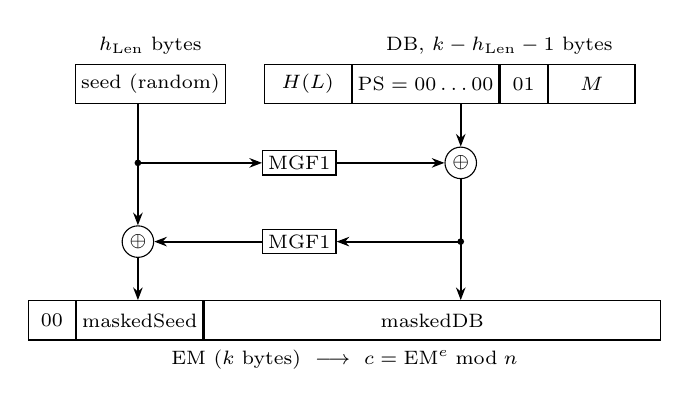
\begin{tikzpicture}[
  font=\scriptsize, x=1cm, y=1cm,
  box/.style={draw, minimum height=5mm, inner sep=2pt, anchor=west},
  op/.style={draw, circle, inner sep=0pt, minimum size=4mm},
  arr/.style={-{Stealth[length=1.6mm]}, thick}
]
  \node[box, minimum width=16mm] (seed) at (0,0) {seed (random)};
  \node[box, minimum width=11mm] (lh) at (2.4,0) {$H(L)$};
  \node[box, minimum width=18mm, right=0pt of lh] (ps) {$\mathrm{PS}=00\dots00$};
  \node[box, minimum width=6mm, right=0pt of ps] (one) {01};
  \node[box, minimum width=11mm, right=0pt of one] (m) {$M$};
  \node[above=0pt of seed] {$\hlen$ bytes};
  \node[above=0pt of ps.north east] {$\mathrm{DB}$, $k-\hlen-1$ bytes};
  \coordinate (sc) at (0.8,0);
  \coordinate (dc) at (4.9,0);
  \node[op] (x1) at (4.9,-1.0) {$\xor$};
  \node[op] (x2) at (0.8,-2.0) {$\xor$};
  \node[draw, inner sep=2pt] (g) at (2.85,-1.0) {MGF1};
  \node[draw, inner sep=2pt] (h) at (2.85,-2.0) {MGF1};
  \node[box, minimum width=6mm] (zero) at (-0.6,-3.0) {00};
  \node[box, minimum width=16mm, right=0pt of zero] (ms) {maskedSeed};
  \node[box, minimum width=58mm, right=0pt of ms] (mdb) {maskedDB};
  \draw[arr] (sc |- seed.south) -- (x2.north);
  \fill (0.8,-1.0) circle (1.2pt);
  \draw[arr] (0.8,-1.0) -- (g.west);
  \draw[arr] (g.east) -- (x1.west);
  \draw[arr] (dc |- m.south) -- (x1.north);
  \draw[arr] (x1.south) -- (dc |- mdb.north);
  \fill (4.9,-2.0) circle (1.2pt);
  \draw[arr] (4.9,-2.0) -- (h.east);
  \draw[arr] (h.west) -- (x2.east);
  \draw[arr] (x2.south) -- (sc |- ms.north);
  \node[anchor=north] at ($(zero.south west)!0.5!(mdb.south east)$)
     {$\mathrm{EM}$ ($k$ bytes) $\;\longrightarrow\;$ $c=\mathrm{EM}^e \bmod n$};
\end{tikzpicture}
\caption{OAEP encoding as in RFC~8017~\cite{rfc8017}.}\label{fig:oaep}
\end{figure}

Let $k$ be the length of $n$ in bytes, $M$ the message and $L$ an optional
label. OAEP encoding (\cref{fig:oaep}) works as follows:
\begin{enumerate}
  \item Check that $|M| \le k - 2\hlen - 2$.
  \item Build the data block $\mathrm{DB} = H(L) \concat \mathrm{PS} \concat
        \mathtt{01} \concat M$, where PS is enough zero bytes to make DB
        $k - \hlen - 1$ bytes long.
  \item Pick a random seed of $\hlen$ bytes.
  \item Compute $\mathrm{maskedDB} = \mathrm{DB} \xor \mathrm{MGF1}(\mathrm{seed})$.
  \item Compute $\mathrm{maskedSeed} = \mathrm{seed} \xor \mathrm{MGF1}(\mathrm{maskedDB})$.
  \item The encoded message is $\mathrm{EM} = \mathtt{00} \concat
        \mathrm{maskedSeed} \concat \mathrm{maskedDB}$, which is then encrypted
        with textbook RSA.
\end{enumerate}
To decode, the receiver removes the masks in reverse order and checks that
the first byte is zero, that $H(L)$ is correct, and that the zeros are
followed by \texttt{01}. If a ciphertext was tampered with, the result looks
random and these checks fail. Because of the random seed, encrypting the same
message twice gives different ciphertexts.

RSA-OAEP has been proven secure against chosen-ciphertext attacks in the
random oracle model, under the RSA assumption~\cite{fops2001,pointcheval2002}.
An important practical point is that all decoding errors must look the same
to an attacker. Manger~\cite{manger2001} showed that if an attacker can tell
whether the first byte was zero, for example from an error message or from
timing, they can recover the plaintext with roughly $\log_2 n$ queries.

% =====================================================================
\section{Implementation}\label{sec:impl}

\subsection{Structure}

Our implementation is a Python package called \code{rsaoaep}. It only uses
the standard library: \code{secrets} for random numbers, \code{hashlib} for
SHA-2 and SHA-3, and \code{hmac} for one constant-time comparison. The rest,
including all the number theory and the padding, is our own code.
\Cref{tab:modules} shows the modules. Users can call
\code{generate\_keypair}, \code{encrypt} and \code{decrypt} from Python, or
use the command-line tool, which stores keys as JSON files and ciphertexts as
base64. On macOS and Linux, private key files are created with owner-only
permissions. A demo script encrypts and decrypts some example text, JSON and
CSV files, or a text or file given by the user.

\begin{table}[t]
\centering
\caption{Modules of the \code{rsaoaep} package.}\label{tab:modules}
\scriptsize
\begin{tabular}{@{}ll@{}}
\toprule
Module & What it does \\
\midrule
\code{math\_utils.py}   & gcd, extended gcd, modular inverse, int/byte conversion \\
\code{primality.py}     & trial division, Miller--Rabin, prime generation \\
\code{rsa\_core.py}     & key generation, RSA encryption and decryption \\
\code{mgf1.py}          & MGF1 mask generation function \\
\code{oaep.py}          & OAEP encoding and decoding \\
\code{types.py}, \code{serialization.py} & key classes; saving and loading keys as JSON \\
\code{exceptions.py}    & error types \\
\code{cli.py}, \code{benchmark.py} & command-line tool; benchmarks \\
\bottomrule
\end{tabular}
\end{table}

\subsection{Primes and Keys}

To generate a $k$-bit prime, we take $k$ random bits from
\code{secrets.randbits} and set the highest bit (so the number really has $k$
bits) and the lowest bit (so it is odd). The candidate is checked by trial
division with the primes up to 37 and then by \cref{alg:mr} with 40 rounds.
If it fails, we try a new random candidate.

\code{generate\_keypair} generates two primes of half the key size each. It
starts again if $p = q$, if $n$ is one bit too short, or if
$\gcd(e, \varphi(n)) \ne 1$. Then it computes $d$ with our extended Euclidean
algorithm. By default we use $e = 65537$ and 2048-bit keys. Keys shorter than
528 bits are rejected, since with SHA-256 the modulus needs at least
$2 \cdot 32 + 2 = 66$ bytes. The private key only stores $(n, e, d)$.

\subsection{OAEP and Hash Functions}

\code{oaep\_encode} follows the steps of RFC~8017, and the random seed
comes from the \code{secrets} module. \code{decrypt} first checks that the ciphertext
has the correct length and is smaller than $n$, then computes $c^d \bmod n$
and calls \code{oaep\_decode}. The start of the decoding function looks like
this:

\begin{lstlisting}
def oaep_decode(encoded: bytes, label: bytes = b"") -> bytes:
    if len(encoded) < 2 * HASH_LENGTH + 2: raise DecryptionError("decryption failed")
    if encoded[0] != 0:                    raise DecryptionError("decryption failed")
    ...  # unmask seed and DB, then check label hash, zero padding and 0x01
\end{lstlisting}

All errors use the same exception and message, and the label hash is
compared in constant time. However, the check of the first byte returns
before anything else is computed, which we come back to in \cref{sec:timing}.

The hash function is set by one constant, \code{HASH\_NAME = "sha256"}.
Since \code{hashlib} has SHA-2 and SHA-3 with the same interface, we only
need to change this one string (e.g.\ to \code{"sha3\_256"}) to use SHA-3.

\subsection{Testing}

We have 39 tests (\code{pytest}), and all of them pass. They cover the
number theory functions (e.g.\ $17^{-1} \bmod 3120 = 2753$ from the example
above), primes and composites such as 341 and 561, MGF1, OAEP with the
longest allowed message and one byte more, round trips through JSON key
files, the CLI and the demo, file permissions of private keys, and invalid
inputs such as wrong labels, changed ciphertexts and too-small key sizes. As
RFC~8017 has no SHA-256 test vectors for OAEP, we also checked that our code
works together with the PyCryptodome library in both directions.

% =====================================================================
\section{Results}\label{sec:results}

All measurements were done on one machine (a Linux aarch64 virtual machine
running on one of our Apple-silicon laptops, Python 3.10). The script
\code{report/experiments/report\_experiments.py} in our repository repeats
all of them.

\subsection{Correctness}

For SHA-256, SHA-512, SHA3-256 and SHA3-512 we encrypted 50 random messages
with random labels using a 2048-bit key, both with our code and with
PyCryptodome, and decrypted each with the other library. All 400 round trips
worked. The longest message that fits is 190 bytes for the 256-bit hashes
and 126 bytes for the 512-bit hashes. OAEP encoding took about
11--12\,\textmu s for every hash, so the choice between SHA-2 and SHA-3 does
not really matter for speed. When we encrypted the same message 1000 times,
we got 1000 different ciphertexts.

\subsection{Performance}

\Cref{fig:perf} and \cref{tab:bench} show our timings. Encryption is very
fast (below 0.4\,ms) because $e = 65537$ is small. Decryption uses the large
exponent $d$ and takes from 2.2\,ms (1024 bits) up to 104\,ms (4096 bits).
Key generation is by far the slowest operation, and its time varies a lot,
because the number of candidates needed to find a prime is random. At 4096
bits a single key took anywhere between 2.1 and 16.1 seconds.

\begin{figure}[t]
\centering
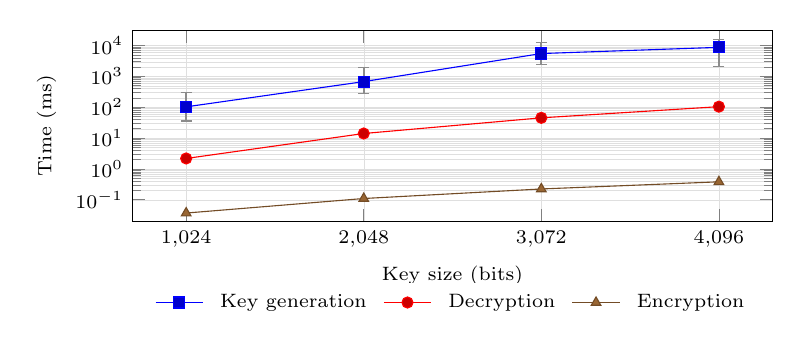
\begin{tikzpicture}
\begin{axis}[
  width=0.8\textwidth, height=4.0cm,
  xlabel={Key size (bits)}, ylabel={Time (ms)},
  ymode=log, xtick={1024,2048,3072,4096}, ymin=0.02, ymax=30000,
  ytick={0.1,1,10,100,1000,10000},
  legend style={font=\scriptsize, at={(0.5,-0.32)}, anchor=north,
    legend columns=3, draw=none, column sep=4pt},
  legend cell align=left,
  tick label style={font=\scriptsize}, label style={font=\scriptsize},
  grid=both, grid style={line width=.1pt, draw=gray!25},
]
\addplot+[mark=square*, error bars/.cd, y dir=both, y explicit,
  error bar style={black!45, line width=0.6pt}] coordinates {
  (1024,102.69)  += (0,194.25) -= (0,67.02)
  (2048,675.75)  += (0,1303.40) -= (0,399.38)
  (3072,5497.16) += (0,7262.48) -= (0,3142.06)
  (4096,8744.73) += (0,7373.47) -= (0,6614.14)};
\addplot+[mark=*] coordinates {
  (1024,2.173) (2048,14.021) (3072,45.188) (4096,104.140)};
\addplot+[mark=triangle*] coordinates {
  (1024,0.0369) (2048,0.1093) (3072,0.2229) (4096,0.3801)};
\legend{Key generation, Decryption, Encryption}
\end{axis}
\end{tikzpicture}
\caption{Median times (log scale). The bars show the fastest and slowest key
generation.}\label{fig:perf}
\end{figure}

\begin{table}[t]
\centering
\caption{Median times in milliseconds. Key generation was repeated $N$
times; encryption and decryption 200 times (60 times for 4096
bits).}\label{tab:bench}
\scriptsize
\begin{tabular}{@{}rrrrr@{}}
\toprule
Key size & $N$ & Key generation & Encryption & Decryption \\
\midrule
1024 & 30 &  102.7 & 0.037 &   2.17 \\
2048 & 20 &  675.7 & 0.109 &  14.02 \\
3072 & 10 & 5497.2 & 0.223 &  45.19 \\
4096 & 12 & 8744.7 & 0.380 & 104.14 \\
\bottomrule
\end{tabular}
\end{table}

\subsection{Prime Generation}

We counted how many candidates were needed to find each prime
(\cref{tab:primes}). The averages are close to the prediction from
\cref{eq:pnt}, for example 354 versus 355 for 1024-bit primes. (The 1536-bit
average is a bit higher, but we only had 60 samples and the spread is very
large.) About 70\% of the candidates were removed by trial division. None of
the composites that reached Miller--Rabin survived even the first round, so
most of the testing time is spent on the 40 rounds for the prime that is
finally accepted (about 85\,ms for a 1024-bit prime).

\begin{table}[t]
\centering
\caption{Candidates needed per prime, compared with $k \ln 2 / 2$.}\label{tab:primes}
\scriptsize
\begin{tabular}{@{}rrrrr@{}}
\toprule
Bits $k$ & Primes & Average candidates & Predicted & Removed by trial division \\
\midrule
512  & 300 & 189.3 & 177.4 & 70.0\% \\
1024 & 150 & 353.7 & 354.9 & 70.2\% \\
1536 &  60 & 642.6 & 532.3 & 70.3\% \\
\bottomrule
\end{tabular}
\end{table}

While doing this, we noticed that key generation often throws away a pair of
primes. Since only the highest bit of $p$ and $q$ is set, their product
sometimes has one bit too few, and the pair has to be generated again. If
$p$ and $q$ are roughly uniform, this happens with probability $2\ln 2 - 1
\approx 39\%$. We measured 37--38\% (200 keys at 1024 bits and 40 keys at
2048 bits), so on average key generation does about 60\% more work than
needed.

\subsection{Miller--Rabin Error Rates}

We also wanted to see how close real numbers come to the bound of $1/4$
strong liars. For some well-known composites we counted the strong liars
among all bases $a \in [2, n-2]$, or sampled 200{,}000 random bases for the
large ones (\cref{tab:mr}). The Carmichael number 561 fools the Fermat test
for 318 bases but Miller--Rabin for only 8. The two large numbers in the
table pass Miller--Rabin for all prime bases up to 7 and 23 respectively, so a
version with these fixed bases would accept them as prime. For them the
fraction of liars is basically exactly $1/4$. Our implementation, which uses
random bases, still rejected both numbers in 1000 out of 1000 tries.

\begin{table}[t]
\centering
\caption{Fraction of bases that are strong liars. $^\dagger$Estimated from
200{,}000 random bases.}\label{tab:mr}
\scriptsize
\begin{tabular}{@{}rlr@{}}
\toprule
$n$ & Note & Strong liars \\
\midrule
561        & Carmichael number ($3\cdot11\cdot17$) & 1.4\% \\
2047       & fools base 2 ($23\cdot89$) & 11.7\% \\
1373653    & fools bases 2, 3 ($829\cdot1657$) & 18.7\% \\
3215031751$^\dagger$ & fools bases 2, 3, 5, 7 & 24.8\% \\
3825123056546413051$^\dagger$ & fools all prime bases up to 23 & 25.0\% \\
\bottomrule
\end{tabular}
\end{table}

\subsection{Timing of Decoding Errors}\label{sec:timing}

Because of the early return mentioned in \cref{sec:impl}, we checked
whether different decoding errors take different amounts of time. We made
three 2048-bit ciphertexts: one where the decrypted first byte is not zero,
one where it is zero but the rest is random (so the label check fails), and
a valid one. \code{oaep\_decode} alone took 0.17\,\textmu s for the first,
11.0\,\textmu s for the second and 14.5\,\textmu s for the valid one, so the
first type of error is clearly faster. When timing the whole \code{decrypt}
function, the difference is only about 20\,\textmu s out of 14.6\,ms, which
is smaller than the normal variation between runs (about 170\,\textmu s).
With enough repeated measurements an attacker could probably still see the
difference, which is exactly the information Manger's
attack~\cite{manger2001} needs.

% =====================================================================
\section{Discussion}\label{sec:discussion}

The implementation works correctly and follows the standard, which we
confirmed by testing it against PyCryptodome with both SHA-2 and SHA-3. Our
measurements also match the theory quite well. Still, it is a proof of
concept and should not be used for real data. The main problems we found are:
\begin{itemize}
  \item \emph{Timing leak in decoding.} The first-byte check should not
    return early. All checks should be computed and combined at the end.
  \item \emph{Python arithmetic is not constant time.} Python's \code{pow}
    can leak information about $d$ through timing. Real libraries use
    constant-time arithmetic and \emph{blinding} (decrypting $c \cdot r^e$
    for a random $r$ and removing $r$ afterwards).
  \item \emph{No CRT.} Because $p$ and $q$ are not stored, we cannot use the
    Chinese Remainder Theorem for decryption. In a quick test this made
    decryption about $3.5\times$ faster (4.0 instead of 14.0\,ms at 2048 bits).
  \item \emph{Wasted primes.} Setting the two highest bits of $p$ and $q$
    would avoid throwing away 39\% of the prime pairs. FIPS~186-5~\cite{fips1865}
    also requires $p$ and $q$ not to be too close to each other, which we do
    not check, and allows fewer Miller--Rabin rounds than our 40.
  \item \emph{Key storage.} Private keys are saved as unencrypted JSON files.
\end{itemize}

RSA-OAEP can only encrypt short messages (190 bytes for a 2048-bit key with
SHA-256). In practice it is used to encrypt a random symmetric key, which
then encrypts the actual data. Our demo only encrypts small files for this
reason.

\paragraph{Open problems.} The security proof of OAEP only works in the
random oracle model, where the hash function is treated as a perfectly
random function, and the proof is not tight~\cite{pointcheval2002}. A more
practical problem is that Shor's algorithm~\cite{shor1997} could factor RSA
moduli on a large quantum computer. Because of this, RSA is expected to be
replaced by post-quantum schemes in the long run.

% =====================================================================
\section{Conclusion}

We implemented RSA-OAEP from scratch, including prime generation with
Miller--Rabin, key generation, MGF1 and OAEP with SHA-2 or SHA-3. The
implementation passes all tests and works together with PyCryptodome. Our
experiments agreed with the theory: the number of candidates per prime
matched the prime number theorem, and the worst composites reached the
Miller--Rabin bound of $1/4$. We also found some weaknesses, mainly a timing
difference in OAEP decoding. The project showed us that a correct
implementation is not automatically a secure one, and that details such as
padding and error handling are as important as the mathematics behind RSA.

% =====================================================================
\bibliographystyle{splncs04}
\bibliography{references}

% =====================================================================
\appendix

\section{Reproducing the Results}

From the repository root (Python 3.9 or newer; use \code{python} instead of
\code{python3} in an activated Windows environment):
\begin{lstlisting}[language=bash]
python3 -m pip install -e ".[dev]"
python3 -m pytest                                  # 39 tests
python3 scripts/run_demo.py                        # demo with example files
python3 -m pip install pycryptodome && python3 scripts/reference_validation.py
PYTHONPATH=src python3 report/experiments/report_experiments.py \
    env random hashes keygen:1024 keygen:2048 mr timing crt \
    prime:512 prime:1024 prime:1536 bench:1024 bench:2048 bench:3072 bench:4096
\end{lstlisting}
The results are written to \code{report/experiments/results\_*.json}.

\section{Additional Measurements}

\paragraph{Second machine.} We also ran our benchmark script
(\code{run\_benchmarks.py}, 3 repeats) directly on macOS (arm64, Python
3.15). The median times for 1024, 2048 and 3072 bits were 48.9, 1100.7 and
3635.1\,ms for key generation, 0.071, 0.153 and 0.313\,ms for encryption,
and 2.38, 16.21 and 53.81\,ms for decryption. Decryption is within
10--20\% of \cref{tab:bench}. Encryption is slower there because that script
times only one encryption per key instead of taking the median of 200 runs.

\paragraph{Mean and standard deviation of key generation} (ms):
$126.9 \pm 72.4$ (1024 bits), $879.0 \pm 520.4$ (2048), $6409.5 \pm 3445.7$
(3072) and $8600.2 \pm 4564.6$ (4096).

\paragraph{More Miller--Rabin data.} Other composites we checked
(strong-liar fraction): 341: 14.2\%, 703: 22.9\%, 1729: 9.3\%,
8911: 20.0\%. A single Miller--Rabin round rejected all 20{,}000 random
512-bit composites without small factors that we tried.

\end{document}
